\documentclass[]{article}

\usepackage{graphicx}
\usepackage{url}
\usepackage{amsmath}
\usepackage{amssymb}
\usepackage{amsthm}
\usepackage{hyperref}
%\usepackage[margin=1.5in]{geometry}
\usepackage{microtype}

\renewcommand{\familydefault}{phv}

%opening
\title{Data Management for Distributed Sensor Networks: A Literature Review}
\author{Anthony J. Christe}

\begin{document}

\maketitle


\begin{abstract}
    Sensor networks can benefit from the generally ``unlimited resources'' of the cloud, namely processing, storage, and network resources. This literature review surveys the major components of distributed data management, namely, cloud computing, distributed persistence models, and distributed analytics.
\end{abstract}

\pagebreak

\tableofcontents
\listoffigures
\pagebreak

\section{Introduction} \label{sec:introduction}
The exponential increase in volume, variety, velocity, veracity, and value of data has caused us to rethink traditional client-server architectures with respect to data acquisition, storage, analysis, quality of data, and governance of data. With the emergence of Internet of Things (IoT) and increasing numbers of ubiquitous mobile sensors such as mobile phones, distributed sensor networks are growing at an unprecedented pace and producing an unprecedented amount of streaming data. It's predicted by the European Commission that IoT devices will number between 50 to 100 billion devices by 2020\cite{6072197}.

The size of sensor networks is quickly growing. BBC Research provides figures that the market share for sensor networks in 2010 was \$56 billion and was predicted to be closer to \$91 billion by the end of 2016 \cite{zaslavsky_sensing_2013}. Data generated from the IoT are surpassing the compute and memory resources of existing IT infrastructures. \cite{chen_big_2014}. Not only is the size of data rapidly exploding, but data is also becoming more complex. Data from sensor networks is often semi-structured on unstructured with data quality issues. 

Sensor networks can benefit from the generally ``unlimited resources'' of the cloud, namely processing, storage, and network resources. We believe that by leveraging cloud computing, distributed persistence models, and distributed analytics, it's now possible to provide a platform that is able to meet the demands of the increasing distributed sensor market and the increasing volume, velocity, variety, and value of data that comes along with that. 

This review summarizes the current state of the art surrounding distributed sensor networks and the use of cloud computing as a means for big sensor data acquisition and analysis. In particular, we will define Big Data and review it in the context of sensor networks, review cloud computing and service models related to distributed sensing, discuss modern distributed persistence for Big Data, and modern distributed analytics for Big Data all with an emphasis on acquiring and managing Big Sensor Data.

\subsection{Applications of Distributed Sensor Networks} \label{ssec:applications-of-distributed-sensor-networks}
Zaslaveky et al. \cite{zaslavsky_sensing_2013} cites several examples of distributed sensor networks in-the-wild including: a real-time greenhouse gas detection network deployed across California, real-time structural monitoring such as the St. Anthony Falls Bridge sensor network in Minneapolis, distributed radiation detection in Fukushima, real-time parking space inventory in San Francisco.

Perera et al. in their paper on sensing as a service\cite{perera_sensing_2014} provide three examples of areas distributed sensor networks would accelerate at. 

First, distributed sensors could be used by cities to optimize waste management which consumes a significant amount of time, money, and labor. Waste management also has many processes including collection, transport, processing, disposal, and monitoring. By collecting and storing sensor data in the cloud from these processes, various interested parties could access sensor data in order to optimize for the current state of the system. As an example, Perera mentions that city council members could optimize garbage routes and collection rates based on the amount of trash available and recycling centers could forecast what to expect based off of the same sensor data. Basically interested parties at all points of the management process could benefit by analyzing data points from IoT devices in a smart city.

Second, Perera mentions that smart agriculture can take advantage of distributed sensor networks and cites the  \textit{Phenonet} project as an example of distributed agricultural sensing which has the ability to monitor plant growth, soil composition, air composition, and pests. A major advantage of this system is that it can supplement traditional research by allowing multiple researchers access to the same data in near real-time.

Third, Perera postulates that environmental management could utilize existing distributed environmental sensors upgraded to communicate with the cloud allowing for data sharing and data fusion among interested parties.

Gerla et al.\cite{gerla_internet_2014} propose an internet of vehicles as a means to autonomous vehicles. By treating vehicles as platforms of thousands of sensors each and by creating dynamic distributed clouds, they hope to allow fleets of vehicles to make autonomous decisions. This model uses distributed clouds based on proximity and peer-to-peer to technologies rather than sending data to a centralized cloud. The real-time nature and the size and amount of sensors makes this an interesting case study.

%% smart grid
One area that shows a lot of promise for distributed sensor networks with centralized management is smart grids. The smart grid is an collection of technologies aiming to advance the electrical grid into the future with respect to intelligent energy distribution and integration of renewable. Electrical grids can benefit by using a large distributed sensor network to collect power consumption, production, and quality information and use that information to control power production and consumption in real-time. 

In some cases, the sensor nodes in smart grids lack powerful local computation abilities, but generally have network connections and sensing capabilities. This makes the cloud a perfect sink of information for analyzing complex power trends from a large scale distributed sensor network for smart grids\cite{botta_integration_2016}.

\subsection{Rest of this Review} \label{ssec:rest-of-this-review}
The rest of this review is structured as follows: Section \ref{sec:big-sensor-data} provides an overview of Big Sensor Data\ref{sec:big-sensor-data}. Section \ref{sec:cloud-computing} will focus on cloud computing and how its concepts can be utilized to manage distributed sensor data. Section \ref{sec:big-data-persistence-models} will examine the current state of the art distributed persistence models with an emphasis on how NoSQL and distributed persistence models can aid in managing distributed sensor data. Section \ref{sec:big-data-analytics} will examine the current state of big data analytics options in the cloud and how these can be utilized for performing analytics on distributed sensor data.

\section{Big Data} \label{sec:big-sensor-data}
Big Data is described using many definitions. Cox, in 1997\cite{cox_managing_1997}, provides us with one of the earliest definitions where Big Data is ``too large to be processed by standard algorithms and software on the hardware one has available to them''. He also mentions that sources for big data collections include data from remote sensors and satellite imaging in the fields of atmospheric sciences, geophysics, and healthcare.

Cox separates Big Data into big data into two categories; namely, \textit{big data collections} and \textit{big data objects}. 

Big data objects are single, very large data sets such as computational models computed from physical phenomena. Big data objects often do not fit in memory or local disks. Big data objects also have adverse affects on bandwidth and latency. Cox looks to moving computation to the data and more advanced segmentation and paging techniques at the OS level to deal with big data objects.

Big data collections contain many smaller objects or even many big objects. Big data collections present their own set of issues including: distributed data, heterogeneous data formats, no platform independent definition, non-local meta-data, large storage requirements, poor locality, and insufficient network resources. 

Cox provides us a useful definition to build on. He also advocates for the development and advancement of operating system constructs for moving data that is too large for memory in and out of memory using stenciling, segmentation, paging, and application controlled segmentation. It's interesting to note that this was before cloud computing and distributed systems, but we are now facing similar problems at the distributed level rather than a local level.

The Apache Hadoop project, in 2010, defined big data as ``datasets which could not be captured, managed, and processed by general computers within an acceptable scope''\cite{chen_big_2014}.

Manyika et al\cite{manyika} in 2011 define big data as ``the amount of data just beyond technology's capability to store, manage, and process efficiently'' essentially making the definition of big data a moving target that is constantly evolving as technology becomes updated.

The Whitehouse report on big data\cite{pcast}, in 2014, defines big data as "data that is so large in volume, so diverse in variety or moving with such velocity,that traditional modes of data capture and  analysis  are  insufficient" and 

Hashem et al.\cite{hashem_rise_2015} build on these previous definition in their 2015 review on Big Data providing the definition by attempting to create a definition that encompasses the spirit of many of the previous definitions. They define big data as ``a set of techniques and technologies that require new forms of integration to uncover large hidden values from large datasets that are diverse, complex, and of a massive scale''.

NIST, in 2015, \cite{nist_big_data_2015} provide multiple definitions relating to big data. NIST defines big data as ``extensive datasets--primarily in the characteristics of volume, variety, velocuty, and/or variability--that require a scalable architecture for efficient storage, manipulation, and analyst. To my knowledge, NIST is the only organization to specify the need of a scalable architecture alongside its definition of big data. NIST next defines the big data paradigm as ``the distribution of data systems across horizontally coupled, independent resources to achieve the scalability needed for the efficient processing of extensive datasets''.

Perhaps one of the most popular definitions of Big Data is characterizing data by ``the four Vs''\cite{hashem_rise_2015}, \textit{volume}, \textit{variety}, \textit{velocity}, and more recently, \textit{value}. 

\subsection{The Three (Four and Five) ``V's"}
The first mention of the three V's was in Laney's 2001 article \textit{3-d data management: controlling data volume, velocity, and variety}\cite{laney20013d}. Laney describes the challenges of managing e-commerce data by categorizing the data challenges into three dimensions. First, we will review Laney's definition of the 3 V's and then we will examine updated, expanded, and more modern interpretations of the three V's and also look at the more recent ``fourth V''.

Volume is the amount of data flowing into a system at any one time. Laney argues that the increased availability of the internet to anyone as an e-commerce platform greatly increases the amount of transactional data stored on server backends. Since data is a tangible asset, organizations may be reluctant to discard the data. At the same time, as the amount of data increases, each individual data point becomes less important. Laney mentions that if organizations are not willing to simply buy more online storage, that they can take the following steps to limit volume growth: implement tiered storage systems, limit data collected to only data required for current organization processes, limit analytics to statistically sampled data, eliminate redundancy in data sources, offload ``cold spots'' to cheaper storage (i.e. tape), and outsorce data management. 

In terms of the increase in data volume, we can look at several statistics starting from the year 2011 and working onwards. According to Gantz et al.\cite{gantz_extracting_2011}, the world wide accumulation of data in 2011  was around 1.8 zettabytes. Then in 2013, during the D11 conference, Meeker presented that this figure had risen to 5 zettabytes across the globe. In 2014, more than 500 million photos were uploaded every day and more than 200 hours of video per minute\cite{pcast}. Tweets generate 12 terabytes of data per day\cite{sharma_extended_2015}.  Perera et al.\cite{perera_sensing_2014} expect with IoT, we could see as many as 1 billion sensors online and generating data by the year 2020. Power meters generate upwards of 350 billion readings annually\cite{sharma_extended_2015}. According to IBM\cite{ibm}, ``90\% of the world's data has been created in the past two years''. 

Velocity is defined by Laney as ``increased point-of-interaction (POI) speed and, consequently, the pace data used to support interactions and generated by interactions'', or more generally, the pace of data arriving and how long it takes to analyze, store, and act on that data. Laney offers several solutions to data velocity in using operational data stored that prioritizes production data, front-end caching, point-to-point data routing protocols, and architecting software in such a way that balances data analysis latency with stated real-time requirements. Some examples of high velocity data include GPS tracking data, web site click streams, social media interactions, and data from mobile sensors\cite{pcast}. Sharma et al.\cite{sharma_extended_2015} also mention that over 5 million trade transactions must be processed daily for fraud detection. 

Laney describes data variety as data that is in ``incompatible formats, non-aligned data structures, and inconsistent data semantics''. Laney's proposed solutions to variety include profiling data to find inconsistencies, a standardized XML data format, interprocess application communication, middlewares on top of ``dumb data'' to provide meaning and intelligent, metadata management, and more advanced indexing techniques. The main reason for the increase in variety of data is due to the prevalence of internet connected devices and the internet of things (IoT) explosion. We now see a wide variety of data that was \textit{born analog} such as sensors measuring our physical world like temperature, solar radiance, power quality, seismic activity, acoustics, etc. We also see much more variety in \textit{born digital data} from the web, social media, government databases, geospatial data, surveys, healthcare, etc\cite{pcast}.

Value is often added as a fourth "V" and represents the value that can only be gained by finding insights into big data. Manika et al. in their McKinsey report\cite{manyika2011big} describe the value of big data after studying the results of long running big data healthcare projects. Value in terms of efficiency and quality of data can be gained from big data using cross correlations and data fusion to gain insights that was not possible before big data. Examples include recommendations from Amazon or Netflix, predict market demand, improve healthcare, and improve security\cite{marr_2015}. Chen et al.\cite{chen_big_2014} believe that value is actually the most important V for big data in that big data often has hidden values that can be extracted using big data analytics. Sharma et al.\cite{sharma_extended_2015} mention that businesses are more and more heavily investing into big data because of the hidden values that could exist.

Finally, veracity has been mentioned alongside the other V's\cite{sharma_extended_2015}. As data volume, variety, and velocity increase, there is a fear that the quality of the data may be hard to ascertain or quantify. Thus, veracity is a measure of the trustworthiness of the data.

\subsection{Features of Big Data}
NIST\cite{nist_big_data_2015} provides us with a list common features of big data. One common feature of big data is associated metadata. Metadata is data about data that includes information about how/when/where the data was collected and processed. Metadata describing the history of data provides for data provenance. This becomes more important as data is transfered between many processes with multiple transformations. Provenance provides a means to track how data was transferred and how it was transformed. Semantic metadata is an attempt at providing metadata with the ability of describing itself. Examples of semantic metadata include the Semantic Web\cite{berners-lee_semantic_2001} and NIST's Big Data Paradigm. 

Another common feature of big data is that it can often be unstructured, semi-structured, or non-relational data. Examples of these types of data include unstructured text, audio, video, and other natural phenomenon that create digitized signals from physical samples. We will review in great detail the big data persistence models in section \ref{sec:big-data-persistence-models} and big data analytical models in section \ref{sec:big-data-analytics} which will examine storage and analysis of unstructured and non-relational data. 

Big data sets tend to exhibit their own features. NIST categorizes big data sets into two categories, \textit{data at rest} and \textit{data in motion}. 

At rest data is data that has already been collected and is stored in cold storage for  non-realtime analysis. The defining feature of data at rest in relation to big data is its volume. It's estimated that by the year 2020, there will be 500 times more data than there was in the year 2011. Big data sets often do not fit on a single server and can be spread out over multiple data centers. Another feature of big data at rest is variety. Data sets can contain data in multiple formats from different domains that in some way need to be integrated to provide value and meaning.  These features of data at rest give rise to the need for distributed big data persistence including shared-disk file systems, distributed filesystems, distributed computing, and resource negotiation.  

In motion data is processed in real-time or near real-time in order to provide immediate feedback. Examples of data in motion include event processing systems from distributed sensors. In motion data can come in the form of data streams. The main feature of data in motion is its velocity. That is the quantity of data that is required to be acquired, persisted, analyzed, and acted upon is large compared to the time window that these operations need to take place. The amount of data that is needed to be acted on in a time window is too much for a single system and has given rise to parallel distributed computing architectures.

Sensor data is a type of big data that has its own defining features which future complicate acquisition, persistence, and analysis \cite{chen_big_2014}. Sensor data often highly correlates both time and location, producing geospatial timeseries data. One of the most common characteristics of sensor data is the amount of noise in the data. Environmental sensing will always include noise because sensor data is born analog\cite{pcast}. Often sensor networks provide data in a large variety of unstructured formats with missing, partial, or conflicting meta-data. Sensor data can also contain a large amount of data redundancy from multiple sensors in similar locations. The problem very quickly becomes a needle-in-the-haystack problem, or more aptly stated, finding the signal in the noise.

\begin{figure}
	\centering
	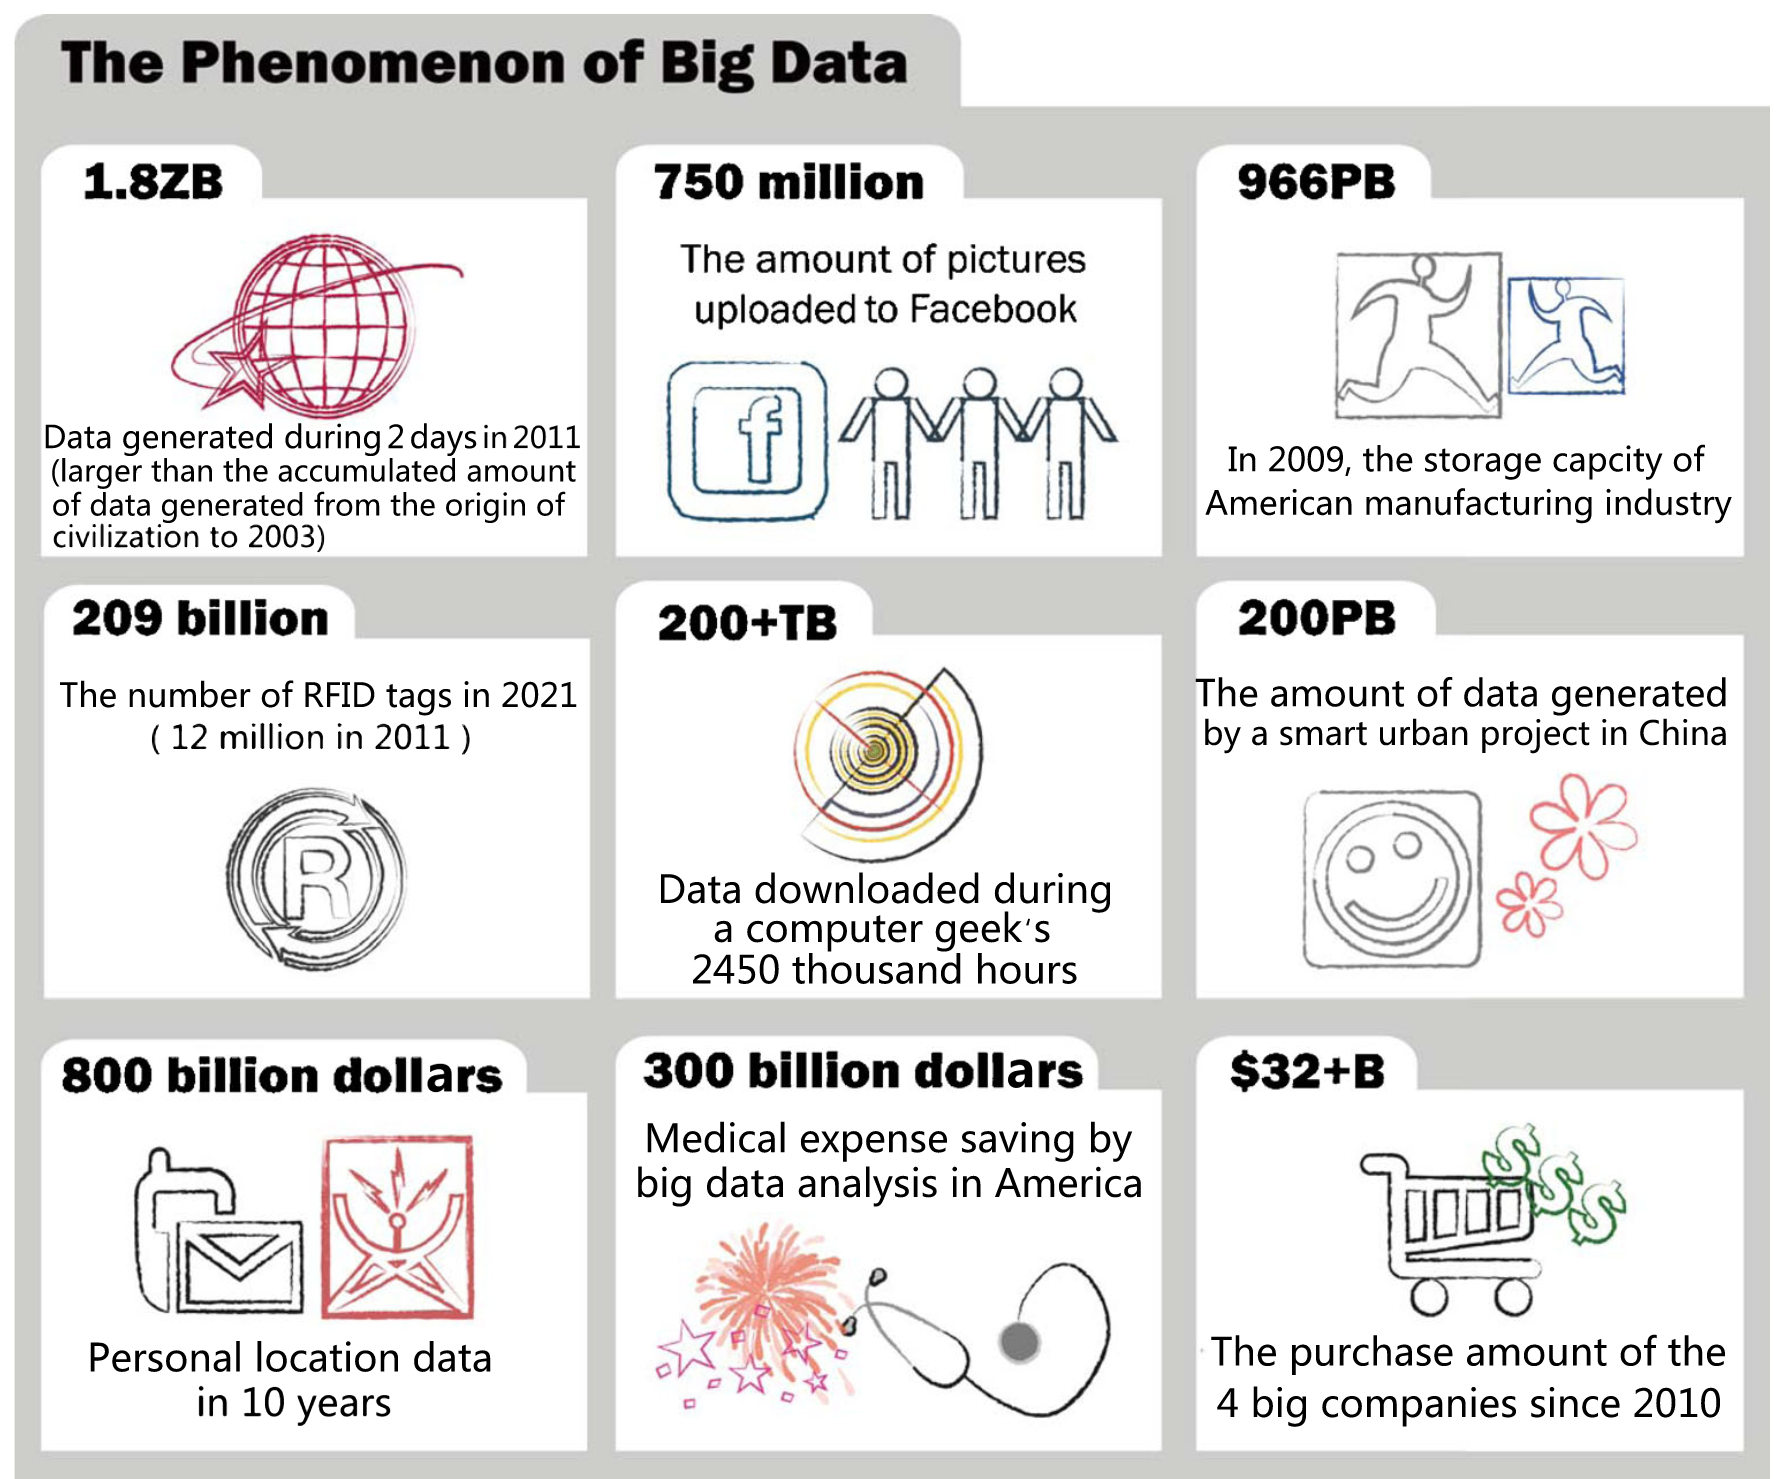
\includegraphics[width=0.8\linewidth]{img/big-data}
	\caption[The Phenomenon of Big Data.]{The Phenomenon of Big Data.\cite{chen_big_2014}}
	\label{fig:big-data}
\end{figure}

Chen shows other examples of big data in figure \ref{fig:big-data}.

\subsection{Examples of Big Data}
Industrial equipment and engines are making use of distributed sensors that generate automated alerts when maintenance is needed\cite{destiche}.

Medicare and Medicaid are using big data predictive analytics to flag fraud before claims are paid to individuals. This has saved over \$115 million dollars a year in fraudulent payout\cite{medicaid}.

Defense Advanced Research Projects Agency (DARPA) has funded various projects for visualization battlefields in real-time and visualization and creating models for traffic flow through road networks, providing valuable intel on where to locate roadside explosives\cite{pcast}.

Researchers at the Broad Institute were able to detect genetic variants in DNA related to schizophrenia \cite{pcast}. The interesting thing about this case is that the variants were not discovered until a large number of samples were analyzed. At low numbers of sample, the variant can not be seen. At intermediate numbers of samples there is a small signal. The genetic  variants become very clear as soon as a certain threshold of data is obtained.

In a review on smart cities and big data authored by Hashem et al.\cite{hashem_role_2016}, the authors review many technologies surrounding big data and how big data can play a role in smart city infrastructures of the future. They found the following areas could benefit from using Big Data in a smart city. 

Smart grids can improve energy generation efficiency by monitoring environmental data, analyzing the power habits of users, and measuring consumption from smart meters\cite{lai2015big}. Smart grids can also make use of big data to perform forecasting of future load generation\cite{al2015applications}. 

Healthcare is another sector that can gain insights on the back of big data. One healthcare project monitored and cross correlated sensors in a neo-natal intensive care unit in order to identify factors that could lead to an infection or early warning signs of infections. Data that was collected included temperatures and heatrates. Analysis allowed doctors to make diagnosis that they would have missed otherwise without big data analytics\cite{ibm_healthcare}.  Analytics of big data in healthcare using big data mining techniques can be used for diagnosing patients, predicting illnesses, and predicting epidemics\cite{roy2007middleware}.

Smart cities can make use of big data to decrease traffic congestion and better plan freight management by analyzing real time traffic sensors and using predictive analysis to determine traffic routes ahead of time\cite{ADMA}. Of course, Google and other companies already do this by analyzing mobile devices to determine and predict traffic congestion.

Hashem et al.\cite{hashem_role_2016} cite several examples of succesful smart city projects in Stockholm, Helsinki, and Copenhagen.


\section{Cloud Computing} \label{sec:cloud-computing}
NIST\cite{mell2011nist} defines cloud computing as ``a model for enabling ubiquitous, convenient, on-demand network access to a shared pool of configurable computing resources (e.g., networks, servers, storage, applications, and services) that can be rapidly provisioned and released with minimal management effort or service provider interaction''.

The major five tenants of cloud computing as defined by NIST are as follows: 

\textit{On-demand self-service} where the user can provision network, storage, and compute capacity automatically without the need for human intervention. In essence, this becomes a virtual shopping mart where to the consumer it appears that virtually unlimited cloud resources are available to chose from and the user (or algorithm) can increase or decrease the utilization of cloud resources at any time.

\textit{Broad network access} where computation capabilities are performed over a network and results are delivered to clients such as mobile devices. 

\textit{Resource pooling} where resources within a cloud such as storage, network, or compute capacity are shared among multiple tenants. This allows for efficient utilization of hardware when generally virtual services are provided to clients. Clients don't necessarily know where their physical hardware is located or provisioned. 

\textit{Rapid elasticity} is the ability to provision or remove cloud resources (i.e. storage, network, or compute resources) at any time from a system as demand on that system either increases or shrinks. Often times a human may not even be involved in making these decisions and this scaling will take place automatically using a set of predefined usage thresholds.

\textit{Measure service} where cloud providers provide a means of metering the compute resources that are used by clients. This provides a transparent means of selling cloud computing resources to clients and clients can always know how much capacity they have consumed.

Even though the NIST definition is starting to show its age, its major tenants are still the underlying foundation of cloud software even today. Many additional service and deployment models have been developed since NIST defined cloud computing, but an understanding of the basic underpinnings is required before exploring the rest of this vast filed.

Cloud computing frameworks can provide on-demand availability and scaling of virtual computing resources for storage, processing, and analyzing of very large data sets in real-time or near real-time. This model makes it possible to build applications in the cloud for dealing with Big Data sets such as those produced from large distributed sensor networks.

By using the cloud as a central sink of data for our devices within a sensor network, it's possible to take advantage of central repositories of information, localized dynamic computing resources, and parallel computations.  With the advent of cheap and ubiquitous network connections, it's becoming easier to do less processing within sensor networks and to offload the work to a distributed set of servers and processes in the cloud\cite{kamburugamuve_framework_2015}.

Cloud computing includes both technical and economical advantages as discussed in \cite{botta_integration_2016}. 

On the economical side, computing resources are pay-per-use. Businesses can dynamically increase or decrease the computing resources they are currently leasing. This makes it possible to utilize massive amounts of computing power for short amounts of time and then scale back resources when demand isn't at its peak. Before cloud computing these same businesses would be required to manage and maintain their own hardware for peak load without the ability to dynamically scale their hardware if the peak load were to increase.

On the technical side, the localization of computing resources provides for a wide variety of benefits including energy efficiency, hardware optimizations, software optimizations, and performance isolation. 

% Other advantages of cloud computing for mobile devices and data
% maybe a brief forway into fog and jungle computing
% The cloud as a collection of services
\subsection{Cloud Computing Service Models} \label{ssec:cloud-computing-service-models}
When discussing cloud computing, it's useful to understand the service models that traditional cloud computing provide. The three major service models as defined by NIST\cite{mell2011nist} are \textit{Infrastructure as a Service} (IaaS), \textit{Platform as a Service} (PaaS) and \textit{Software as a Service} (SaaS).

At the lowest level is  the Infrastructure as a Service (IaaS) model which provides virtual machines that users have the ability to  deploy and manage. Users can install operating systems on these virtual machines and interact with deployed virtual machines as if they were local servers.  Consumers using IaaS have the ability to manage and provision virtual hardware and network resources, but do not need to worry about the underlying hardware or network infrastructures. Other than providing virtual resources, consuming utilizing IaaS still require a decent amount of systems administration knowledge develop, deploy, and secure applications into the cloud using IaaS.

Sitting in the middle of the traditional cloud service models is the Platform as a Service (PaaS)  model. In this service model consumers don't have the ability to interact or provision individual cloud resources such as virtual machines, storage, networking, or compute capacity. Instead, users have the ability to deploy their application to the cloud via custom cloud provides tools or via a cloud provided application programming interfaces (APIs).

At the highest level is the Software as a Service (SaaS) layer. Generally speaking, applications in a SaaS environment are generally provided by the cloud provider. In a SaaS model, users do not have the ability to control their own cloud resources and users do not have the ability to upload their own applications to the cloud. Users do sometimes have the ability to alter the configuration of the software they are interacting with in this model.

Since the original service models were penned, there have been many other types services models introduced. Several of these focus on IoT service layers as noted by Botta et al's\cite{botta_integration_2016}. These include \textit{Sensing as a Service} (S$^2$aaS), \textit{Sensing and Actuation as a Service} (SAaaS), \textit{Sensor Event as a Service} (SEaaS), \textit{Sensor as a Service} (SenaaS), \textit{Data Base as a Service} (DBaaS), \textit{Data as a Service} (DaaS), \textit{Ethernet as a Service} (EaaS), \textit{Idendity and Policy Management as a Service} (IPMaaS), and \textit{Video Surveillance as a Service} (VSaaS).

Some of the above mentioned service models are of particular interest for a survey examining cloud computing and sensor networks. We will examine these in more detail in sections \ref{ssec:sensing-as-a-service}.

\subsection{Sensing as a Service} \label{ssec:sensing-as-a-service}
Sensing as a Service (SaaS or S$^2$aaS) describes ``the process of making the sensor data and event of interests available to the clients respectively over the cloud infrastructure''\cite{dash_survey_2010}. 

The sensing as a service model includes 4 layers\cite{perera_sensing_2014}. Figure \ref{fig:sensing-as-a-service} shows these 4 layers in more detail.

\begin{figure}
    \centering
    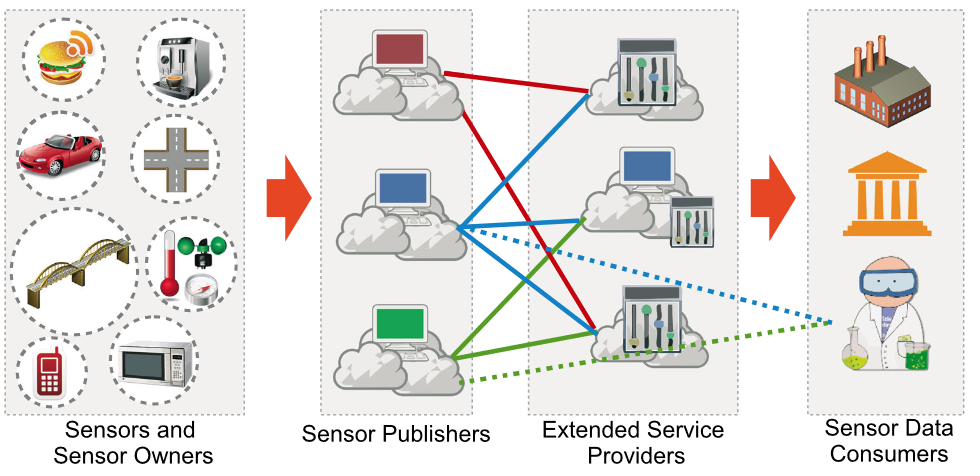
\includegraphics[width=1.0\linewidth]{img/sensing-as-a-service}
    \caption[Sensing as a service layers.]{Sensing as a service layers.\cite{perera_sensing_2014}}
    \label{fig:sensing-as-a-service}
\end{figure}

The \textit{sensor and sensor owners} layer includes physical sensors which can sense an increasingly broad variety of natural phenomena and sensor owners which can be personal, household, private, public, or commercial. Sensor owners have the final say in what data gets to the cloud and who can access the data once it is in the cloud using conditions and restrictions.

The \textit{sensor publishers} (SP) layer manages the detection of online sensors and acts as a middle-man between sensor consumers and sensors and sensor owners. Sensors register with the publisher layer. Sensor data consumers make requests to sensor publishers for specified types of data over specified amounts of time.

The \textit{extended service providers} (ESP) layer builds abstraction on top of sensor publishers. A single ESP can interact with mulitple SPs. ESPs can be used to automatically request data from multiple sensors depending on criteria provided to the ESP. This can be useful if the sensor consumer does not care about the underlying individual sensors but instead queries data at a higher level (i.e. all temperature data within a given polygon).

Finally, the \textit{sensor data consumers} layer consist of data consumers who must register with the ESPs and provide valid digital certificates. Consumers can either deal with SPs directly or deal with ESPs. The benefit to dealing with SPs is reduced cost of communications with the ESP. The benefit of dealing with ESPs is higher level querying to data and the ability to query data across multiple SPs.

I find sensing as a service appealing, but lacking in actual implementation details. To Perera's credit, he does mention quite a few open technological challenges that need filled including architectural designs, sensor configuration, sensor management, data fusion, filtering, processing, storage, and energy consumption.

Rao et al.\cite{rao_cloud_2012} mention several other research challenges for SaaS including the need for a standard distributed computing framework for distributed big sensor data as well as a framework for the real-time monitoring of sensor events.

\subsection{Sensor as a Service} \label{ssec:sensor-as-a-service}
In a Sensor as a Service (SenaaS) \cite{alam_senaas_2010} service model, virtual and physical sensors are combined according to a Service Oriented Architecture. This type of model concerns itself more with the management of distributed sensors than it does with the access, transfer, and governance of data as the sensing as a service model\cite{zaslavsky_sensing_2013}. Figure \ref{fig:sensor-as-a-service} shows the three layers that make up the architecture in the SenaaS model. Sensors and events can be defined and standardized in XML and other serialization formats such as SensorML\cite{sensorml} and OWL\cite{dean_owl_2004}.

\begin{figure}
    \centering
    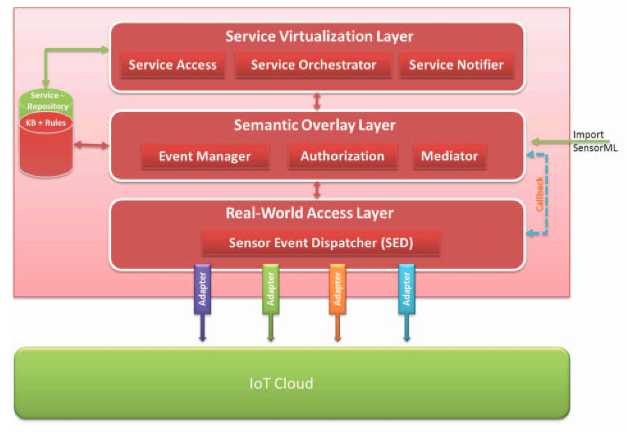
\includegraphics[width=1.0\linewidth]{img/sensor-as-a-service}
    \caption[Sensor as a service layers.]{Sensor as a service layers.\cite{alam_senaas_2010}}
    \label{fig:sensor-as-a-service}
\end{figure}

The \textit{Real-World Access Layer} interfaces to the sensors using adapters which need to be designed for each sensor. Messages from this layer are asynchronously forwarded to the \textit{Semantic Overlay Layer} via callbacks.

The \textit{Semantic Overlay Layer} is responsible for persisting data either in-memory or on disk. This layer also provides for in-memory caching capabilities. Policy based authorization can be implemented in this layer to provide some control over data access.

The \textit{Service Virtualization Layer} provides an abstraction on top of the semantic overlay layer by performing queries based on the access rights of consumers. This layer transforms the results of queries into something that can be consumed by the clients.


\subsection{Cloud Deployment Models} \label{ssec:cloud-deployment-models}
NIST\cite{mell2011nist} provides four types of deployment models in its cloud computing definition: \textit{private cloud}, \textit{community cloud}, \textit{public cloud}, and \textit{hybrid cloud}.

A private cloud is is a cloud where resources are provisioned to a single organization (or multiple parties within a single organization). In this model the organization may deploy their own cloud hardware or use cloud resources provided by a third party.

In a community cloud, resources are provided to a group of organizations that have similar requirements and may be owned and managed by a single organization, multiple organizations, or third parties.

Public clouds provide computing resources to anyone willing to purchase  said cloud resources. Public clouds can be owned and manged by anyone, a government, or any third-party. Generally all hardware in public clouds are managed by the cloud provider.

Hybrid clouds use and provide a combination of the previously mentioned deployment models and can be configured, split-up, and manged in many ways.

Virtual private clouds as described in Botta et al.\cite{botta_integration_2016} provide aspects from both public and private clouds using virtual private network (VPN) technology to allow users to manage specific and often times complicated network technologies.

\subsection{Mobile Cloud Computing} \label{ssec:mobile-cloud-computing}
Mobile devices such as smartphones make fantastic distributed sensors for temporalspatial data. Not only do they carry a wide array of sensors on-board (microphones, barometers, accelerometers, GPS, compasses, cameras, clocks), but they generally have multiple modes of offloading data (WiFi, bluetooth, cellular, SD cards), and support some pre-processing on-board.

TODO: Expand on this more with an emphasis on the broad range of sensors being used by cellular networks..

\subsection{Issues with Cloud Computing} \label{ssec:issues-with-cloud-computing}
The biggest issues facing cloud computing deal with security and privacy. Subashini et al.\cite{subashini_survey_2011} go into the specific security and privacy risks associated with the three major cloud deployment models. The following is largely a review of their work. 

The deployment model that exhibits the most risks in the PaaS layer since this model requires that consumers manage their own virtual machines, deployment of cloud applications, and configuration. Within this model, the following items are of concern. 

Data security is a concern on all deployment models, but especially at the PaaS layer where sensitive data will be stored on remote servers not owned by a client. Since clients manage their own servers in the PaaS layer, they are also required to manage their own data security. Data security issues include cross-site scripting, access control weaknesses, injection attacks, cross-site request forgery, cookie manipulation, hidden field manipulation, insecure storage, and insecure configuration.

Network security becomes an issue when sensitive data is transferred from clients to the cloud backed and visa-versa. If encryption is not used, users could be vulnerable to port scans, ip spoofing, man-in-the-middle attacks, packet sniffing, and more. Even if encryption is used, users can still be vulnerable to packet analysis, insecure SSL configurations, session management weaknesses.

Laws and regulations often require that data not leave or enter certain jurisdictions giving rise to issues of data locality. Users generally do not get to decide where data is stored within a cloud environment as most of those decisions are handled by the cloud provider.

The introduction of distributed systems means that we can no longer make guarantees about data persistence such as ACID (Atomicity, Consistency, Isolation, Durability). Without these guarantees a large amount of data integrity issues surface. We will look at these issues in greater detail when discussion big data persistence models in later chapters.

Data segregation issues occur with multiple virtual resources sharing the same physical resources. Data can be unintentionally leaked or stolen either by attacking the cloud provider multi-tenancy framework or by attacking the virtual servers directly through SQL injection, data validation, and insecure storage.

Large organizations with multiple employees having access to the cloud can create data access issues. Clear policies must be defined, enforced, and updated as to which virtual resources employees have access to. 



At some level, consumers are required to trust that the cloud provider they choose will implement security and privacy best practices within their cloud architecture. This does now however resolve the larger issues of security vulnerabilities within cloud software and their communication components.

% Something about runaway data costs.... there was an issue once of someones AWS key being found and then their servers got pwned and were used for generating bitcoin or something


%%%%%%%%%%%%%%%%%%%%%%%%%%%%%%%%%%%%%%%%%%%%%%%%%%%%%%%%%%
\section{Big Data Persistence Models} \label{sec:big-data-persistence-models}
Traditional storage methods for meta-data and related products has traditionally made use of the filesystem and relational database systems (RDMS).

Big Sensor Data by its nature can be structured, unstructured, large, diverse, noisy, etc. Many of the properties of BSD do not fit nicely into the structured world of traditional RDMSs.

In-order to meet the needs of Big Sensor Data and distributed sensor networks, we look to the ever growing field of NoSQL (not only SQL) and related Big Data storage models. There are multiple types of data models with different use cases. We will review the current players in this field and with a focus on how these technologies could aid in managing Big Sensor Data in the cloud.

According to Song et al.\cite{5980904} an ideal NoSQL data model strives for ``high concurrency, low latency, efficient storage, high scalability, high availability, reduced management and operation costs.'' The challenges of realizing an ideal NoSQL data model however lie in three main areas\cite{chen_big_2014}: consistency, availability, and partition tolerance. 

% Discussions on consistency
Several of the persistence models we review do not support ACID (Atomicty, Consistency, Isolation, Durability). A consequence of this is less than perfect consistency. Consistency issues occur when data is stored in a distributed manner with multiple copies. In situations of server failure (or with systems that support different consistency models), situations can arise where multiple copies of the same resource contain different contents. 

Vogels and Wener\cite{vogels_eventually_2008} explain the main forms of consistency. Assume a record is being updated across multiple servers. With ``strong consistency'', any access of that resource after the update will return the updated result. With ``weak consistency'', subsequent access of that resource is not guaranteed to return the updated result if that access is within a certain ``inconsistency window''. With eventual consistency, the only guarantee you get is that access to the resource will be show up ``eventually'' where eventually can depend on many factors.

% Discussions on availability
As the amount of hardware (servers, switches, \textit{etc}) increases in a distributed system so does the amount of hardware errors. Availability refers to the ability to remain operational even as parts of a distributed system drop in and drop out\cite{chen_big_2014}. Gilbert\cite{gilbert2002brewer} defines availability as ``every request received by a non-failing node in the system must result in a response." He goes on further to point out that this definition does allow for unbounded computation since it's possible to wait for a result that never returns.

% Discussion on partition tolerance
As the amount of hardware increases in a distributed system, the number of communication packets that drops also increases. The ability to maintain service in the face of some amount of drops refers to partition tolerance\cite{chen_big_2014}.

The above ideas are all tied together into the CAP theorem proposed by Brewer\cite{brewer2000towards} which states that in any shared data system, you can only achieve two of the three following properties: Consistency, Availability, or Partition (tolerance). As we review different Big Data architectures, we will examine how they fit into the CAP theorem and what guarantees they provide for these three major areas of distributed data management.

We also believe, ease of use, maturity of the product, and community (or commercial) support should also factor into the comparisons between data models. 

With the above factors in mind, we can begin categorizing and analyzing several major Big Data model solutions.

\subsection{Data Models} \label{ssec:data-models}
\subsubsection{Key-Value}
The simplest data model for distributed storage is likely the Key-Value (KV) data model \cite{weber_nosql_2010}. In this model, every piece of data stored is indexed by a unique primary key. Queries to that item all happen via its key to access the value. Values in a KV system can be treated as blobs and the content of the value is irrelevant to the semantics of KV stores. KV systems are popular due to their simplicity and ease of scaling.

Keys in KV systems are the unit parallelism that provide the main means of concurrency. If you want to guarantee transactions, then keys can be naively sharded across servers. This does now however provide safety of data loss in which case a system will strive to provide replication at the cost if ACID compliance. Stores and requests can usually be achieved in $O(1)$ even in distributed systems\cite{ravendb}.

If the major advantages are simplicity and query response time\cite{chen_big_2014}, the major disadvantage to KV stores is the fact that they lack advanced query capabilities. The only way to query a database is by its unique key. Range based queries, secondary, and tertiary indexes are only supported by a third party systems.

Popular KV based solutions include Dynamo, Riak, Voldemort, Redis, MemcacheDB, Ignite  and others.

Key-Value stores can be useful tools for simple distributed sensor networks that keep track of a handful of non-complex data such as current temperature, current voltage, etc. Issues arise when you want to start recording timestamped data. If timestamped data arrives at irregular intervals, KV stores to not provide range based queries to query on timestamps. Thus, KV stores may be poorly suited for time based sensor data. Finally, KV stores do not provide queries for location based sensor data making it potentially a poor choice for geo-spatial data.

\subsubsection{Document}
Document based data models allow data to be stored in structured documents including KV pairs. The underlying document structure can be anything as long as its structure is something that the store can understand. Common document formats include XML, JSON, YAML, BSON, RavenDB, and others\cite{chen_big_2014}. Documents can also store other documents recursively.

Even though documents are restricted to their underlying structure (i.e. JSON, YAML, etc), document databases do not impose a schema like traditional RDMS databases. This allows for painless transitions of data storage when the underlying data change\cite{sharma_extended_2015}.  This is of special concern with heterogeneous sensor networks which can produce large varieties of data in different and changing formats.

Document based data stores often present less of an impedance mismatch between data structures in a programming language and their underlying representation in the data store. Compared to the way data is structured in a RDMS, it's often easier to understand the underlying data structure in a documented based store. There are many common libraries for converting between documents in a document store and a data structure in a particular programming language. Compared to RDBMS, fields in document stores generally do not normalize their data which also enhances the readability of the underlying data structure\cite{ravendb}.

An advantage that document based stores have over KV stores is that its possible to create more complex queries. Not only can you query on the primary key, but its possible to create queries over any keys in the document including in sub-documents. Indexes can be created on key and sub-keys. Many document based stores provide range and geospatial based queries. This advantage alone makes document based stores a decent choice for distributed sensor data.

Common document based stores include MongoDB, CouchDB, OrientDB, RavenDB, SimpleDB, 

\subsubsection{Graph}
\subsubsection{Wide Column Store}

\subsection{Data Guarentees}
\subsubsection{title}

\subsection{Indexing}


% Provide a small forray into TSDBs

\section{Big Data Analytics} \label{sec:big-data-analytics}

%\section{Privacy}

%\section{Reference Implementations}

%\section{Open Research Question}

\bibliography{litreview}
\bibliographystyle{plain}

\end{document}
